\documentclass[a4paper,12pt]{article}
\usepackage[utf8]{inputenc}
\usepackage[T1]{fontenc}
%\usepackage{setspace}
\usepackage[francais]{babel}
\usepackage{hyperref}
\usepackage{array}
\usepackage{soul}
\usepackage{graphicx}


\renewcommand{\contentsname}{Sommaire}

% Title Page
\title{LICENCE 2 INFORMATIQUE \\ PROJET: PROUVEUR LOGIQUE PROPOSITION}
                                                                          
\author{Z. Zoro-Bi, M.R. Rahli, S. Stefanovski, I.D. Minko Amoa}
\date{ 05 Mai 2017 \\ Encadrant : M. Leclère \\ Responsable: F. Ulliana \\ }


 

\begin{figure}[t]

\includegraphics[width=50mm]{index.png}
 

\includegraphics[width=100mm]{image.png}

\end{figure}

\begin{document}


\maketitle

 

\pagebreak
\begin{abstract} 

Ce document a pour but de décrire le déroulement de notre projet d'informatique PROUVEUR LOGIQUE  PROPOSITION.\\
Le but de ce projet est de réaliser un système de démonstration de preuve.\\
On s'est restreint au domaine de la logique des propositions.\\\\


Ce rapport contient l'ensemble des éléments du projet.Tout d'abord nous présenterons le  domaine de l'informatique dans lequel se situe notre projet.
Ensuite nous présenterons le domaine précis sur lequel nous avons travaillé.
Puis nous décrirons le fonctionnement de notre projet dans son ensemble ainsi que les éléments qui prouvent le bon fonctionnement de celui-
ci.\\\\

La dernière partie a pour objectif de présenter l'ensemble des apports du sujet: d'un point de vue technique,pédagogique,puis personnel.
Enfin nous ferons le point sur les difficultés rencontrées lors du projet.\\\\

Nous espérons que vous prendrez autant de plaisir à lire ce rapport que nous en avons pris
durant tout le déroulement de ce projet.





\end{abstract}

\pagebreak

\tableofcontents

\pagebreak
\section{Présentation du domaine de l'informatique dans lequel se situe notre projet}
Le projet s'insère dans le domaine de la logique.Nous vous parlerons de la syntaxe utilisée dans la logique des propositions ainsi 
que des différentes définitions dont on a besoin pour la compréhension de ce projet.

\subsection{La syntaxe de la logique des propositions}
\begin{itemize}
\item Soit l'ensemble des mots définis sur l'alphabet S$\cup$C$\cup$D$\cup$L où : 

\subitem S est un ensemble dénombrable de symboles propositionnels notés en lettre minuscule dans les exemples S=\{p,q,r...\} 
\subitem C=\{$\neg$,$\wedge$,v,$\rightarrow$,$\leftrightarrow$\} est l'ensemble des connecteurs logiques non (négation),   et (conjonction),   ou (disjonction),   implique /si-
alors (implication),  équivalent/si-et-seulement-si  (équivalence)
\subitem D=\{(,)\} est un jeu de parenthèses
\subitem  L=\{$\top$,$\bot$\} les constantes logiques  Top(True/Vrai), Bottom(Absurde).
\end{itemize}
Nous retrouvons au niveau des connecteurs logiques des règles de priorité.\\
$\neg$ est prioritaire sur  $\wedge$,$\vee$ qui sont prioritaires sur $\rightarrow$ $\leftrightarrow$. 
\subsection{Remarques}

  Convention:
  \begin{itemize}
 \item Les majuscules dénotent des formules bien formées:\\
 P,Q,R...
 \item Les miniscules dénotent des symboles propositionnels:\\
 p,q,r..
 \item Attention:
 \item Tout symbole propositionnel est une proposition.
 p est à la fois une formule bien formée de PROP($\{$p,q$\}$) et un symbole de {p,q}
 \item Le contraire n'est pas vrai ! 
 (p $\wedge$ q) est une formule bien formée de PROP($\{$p,q$\}$) mais n'est pas un symbole\\
 \item Une formule réduite à un symbole propositionnel ou aux constantes logiques $\top$ ou $\bot$
 est appelée une formule atomique ou atome.
 \end{itemize}

\subsection{Différentes syntaxes}
\begin{itemize}
 \item Différentes formules bien formées peuvent avoir la même sémantique\\
 $\rightarrow$  les connecteurs sont redondants\\
 Ex.(P$\leftrightarrow$Q) $\equiv$ ((P$\rightarrow$Q) $\wedge$ (Q$\rightarrow$P))
 \item Dans les démonstrations, on pourra se limiter aux seuls connecteurs $\neg$,$\wedge$,$\rightarrow$ en traitant les autres
 comme des macros (des raccourcis d'écriture):
 \item $\bot$ pour (P$\wedge$ $\neg$P)
 \item $\top$ pour $\neg\bot$
 \item (P$\vee$Q) pour $\neg$($\neg$P $\wedge$ $\neg$Q)

\end{itemize}

\subsection{Les Formules bien formées}

On définit PROP(S),l'ensemble des formules bien formées de la logique des propositions(ou propositions), construites sur S par induction : (base) S $\cup$ {$\top$, $\bot$}(cons)  
Soit P et Q des mots de (S$\cup$C$\cup$D$\cup$L)*, on dispose de 5 règles de construction 
r1(P) = $\neg$P 
r2(P,Q) = (P $\wedge$ Q)  
r3(P,Q) = (P $\vee$ Q) 
r4(P,Q) = (P $\rightarrow$ Q) 
r5(P,Q) = (P $\leftrightarrow$ Q).


\subsection{Les littéraux}

Un littéral est une formule bien formée réduite à un symbole propositionnel ou à la négation d'un symbole propositionnel. 
On parle de littéral positif (ex. p) ou de littéral négatif (ex : $\neg$p ).
On parle du littéral opposé d'un littéral donné (ex : $\neg$p et p sont opposés).

\subsection{Les Séquents}
Un séquent est un ensemble comprenant un ensemble d'hypothèses et une conclusion étant une formule bien formée.
On suppose fixé un ensemble de formules logiques. Un séquent est une expression de la forme suivante
H1, . . . ,Hm$\vdash$C1
C’est à dire (formellement) deux suites finies de formules, les hypothèses et la conclusion du séquent.

\subsection{Les règles d'inférences}
Dans un système logique, les règles d'inférence sont les règles qui fondent le processus de déduction, de dérivation ou de démonstration. 
L'application des règles sur les axiomes du système permet d'en démontrer les théorèmes.
Une règle d'inférence est une fonction qui prend un n-uplet de séquents et 0-uplet ou n-uplet de séquents. Les formules arguments sont appelées « les prémisses » et la formule retournée est appelée la « conclusion ». 
Si l'ensemble des prémisses est vide, alors la conclusion est appelée un « théorème » ou un « axiome » de la logique.
Un axiome désigne une proposition indémontrable utilisée comme fondement d’un raisonnement ou d’une théorie mathématique.


\subsection{Notions utiles}
 Prenons par exemple cette formule bien formée: $\neg$($\neg$q$\wedge$(p$\vee$q$\vee$p$\rightarrow$q))$\rightarrow \neg$p)\\
 voici ci-dessous sa représentation dans un arbre binaire.\\
\begin{center}
 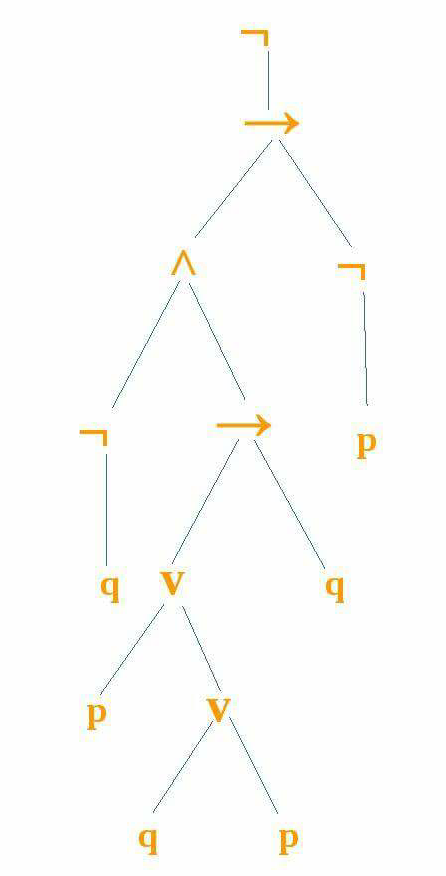
\includegraphics[width=30mm]{image1.png}
 \end{center}
 Les notations préfixée,post-fixée,ont l'avantage de ne pas nécessiter de parenthèses \\
 PREFIXEE (Racine, Fils Gauche, Fils Droit) :    $\neg$ $\rightarrow$ $\wedge$ $\neg$ q $\rightarrow$ $\vee$ p $\vee$ q p q $\neg$ p \\ 
 POST-FIXEE (Fils Gauche, Fils Droit, Racine) :  q  $\neg$  p  q  p  $\vee$  $\vee$ q  $\rightarrow$  $\wedge$ p $\neg$ $\rightarrow$ $\neg$\\
 On peut ajouter à ces notations, la notation infixée.\\
 INFIXEE(Fils Gauche,Racine,Fils Droit) : q $\neg$ $\wedge$ p $\vee$ q $\vee$ p $\rightarrow$ q $\rightarrow$ $\neg$ $\neg$ p

 
 
 \section{Présentation du domaine précis sur lequel nous avons travaillé}
 
 
Comme s'énonce le projet, le domaine précis étudié se situe au niveau de la démonstration de propriétés de formules bien formées.
Nous vous rappelons que le but du projet c'est de développer un logiciel qui est capable étant donné un séquent de savoir s'il est prouvable ou pas. 
En logique de proposition plusieurs méthodes(règles) sont utilisées pour la démonstration de la propriété de la formule bien formée.
dont la méthode de résolution et la méthode des tableaux...
Nous utilisons 14 règles appelées règles d'inférence qui permettent la réalisation su système de preuve.
Notre programme utilise toutes ces règles dans un ordre précis et bien définis.\\
Ces règles sont énumérées dans cet ordre:BS1,BS2,DB1,DB2,DR1,DR2,\\DR3,DR4,DR5,DR6,DR7,DR8,CNJ,DED\\
Dans le cadre de notre projet $\neg$ est représenté par "!",$\wedge$ est représenté par "\&",$\rightarrow$ est représenté par ">".


\subsection{Les preuves de la logique}
Le système de preuve consiste à automatiser les preuves de la logique. 

Les preuves qu'on vise sont de la forme  hypothèses à hypothèses entraîne conclusion qu'on a appelé séquent.

Dans le cas de notre projet les hypothèses et la conclusion sont des formules de la logique des propositions qui se représentent de la forme
connecteur et symbole propositionnel ou symbole propositionnel,connecteur,symbole propositionnel.


on se base sur ces règles  pour pouvoir prouver la propriété d'une formule dans un 
ordre respecté.

\subsection{Exemple de preuve}
Nous avons le sequent suivant à prouver (il est bien de remarquer que celui-ci ne possède pas d'hypothèses). \newline
$\vdash$ P $\rightarrow$ $\neg\neg$ P\\

Après l'application de la règle DED on obtient:

P $\vdash$ $\neg\neg$ P\\

On applique la règle DR7\\

P $\vdash$ P \\

D'après la règle BS2 le séquent a été prouvé.




\section{Processus du projet}

\subsection{Diagramme de Gantt}
\begin{center}
 


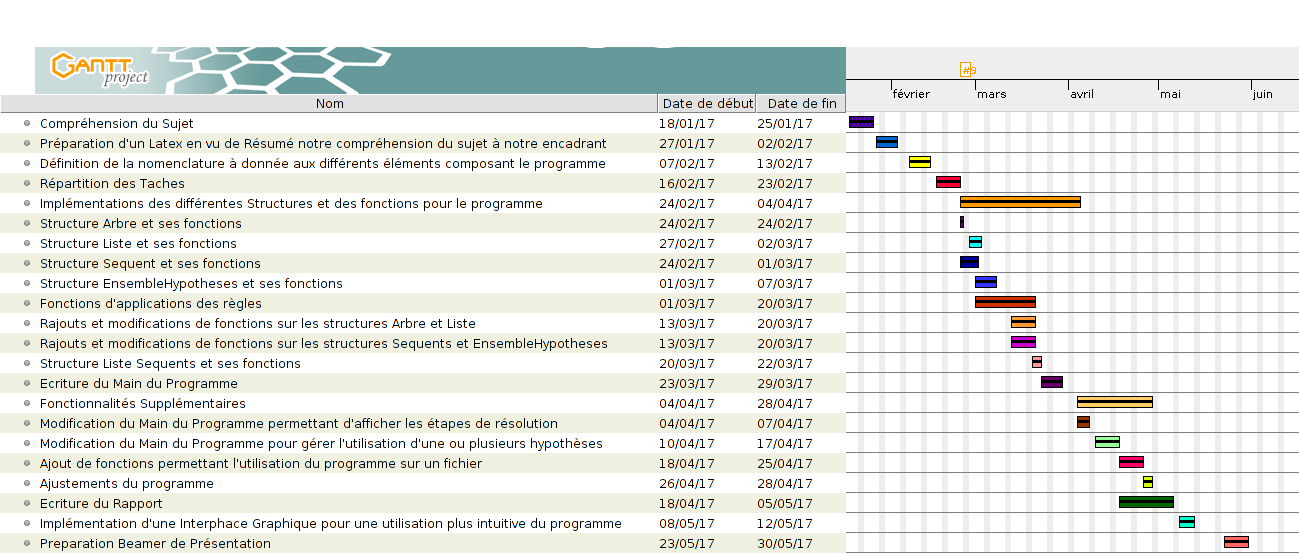
\includegraphics[width=150mm,\texwidth,left]{ii.png}

\end{center}
Nous commencerons par vous donner un résumé de toutes les fonctions utilisées dans le programme afin que vous en 
ayez un aperçu.\\



\includegraphics[width=167mm]{uml.png}\\

Le programme se déroule comme suit:
\begin{itemize}
 \item L'utilisateur rentre un séquent dans le terminal Unix ou dans un fichier texte.
 \item Si on prend la première méthode on peut avoir plusieurs formules dans un fichier On précise au programme le fichier contenant les séquents à prouver et le fichier contenant les règles à appliquer pour la résolution de ces séquents.
 \item Si le séquent a été mis dans un fichier texte,l'utilisateur devra rentrer le nom de celui-ci dans le terminal pour en informer le programme.
 \item Ensuite la syntaxe du séquent entré par l'utilisateur est vérifiée.Dans le cas où l'utilisateur n'a pas respecté les règles de construction d'un séquent,il en est informé et le programme
 lui demande d'en rentrer un autre.Le symbole "$\vdash$" permet à l'ordinateur de faire la différence entre l'ensemble d'hypotheses et la conclusion. Si le séquent ne possède aucun élément avant le symbole "$\vdash$", alors le programme considérera que le séquent n'a pas d'hypothèses.\\
 \item Le programme récupère ce que l'utilisateur a rentré et vérifie si chacune des règles est applicable.Deux possibilités s'offrent à nous:
 \subitem Soit une ou plusieurs règles sont applicable alors: on applique la première règle applicable.Le programme répète la vérification de l'application des règles sur le ou les séquents obtenus, 
 jusqu'à ne plus pouvoir en appliquer une.Il s'arrête aussi dans le cas où il n'y a plus de séquent à prouver.Le ou les derniers séquents obtenus sont donnés par le programme à la fin de la preuve.
 \subitem Soit aucune des règles n'est applicable et l'utilisateur en est informé. 
 
 
 
 
 
 
\end{itemize}

\subsection{Description des fonctions les plus importantes utilisées dans le programme}
\subsubsection{La fonction qui permet de la saisie d'un séquent sur le terminal}
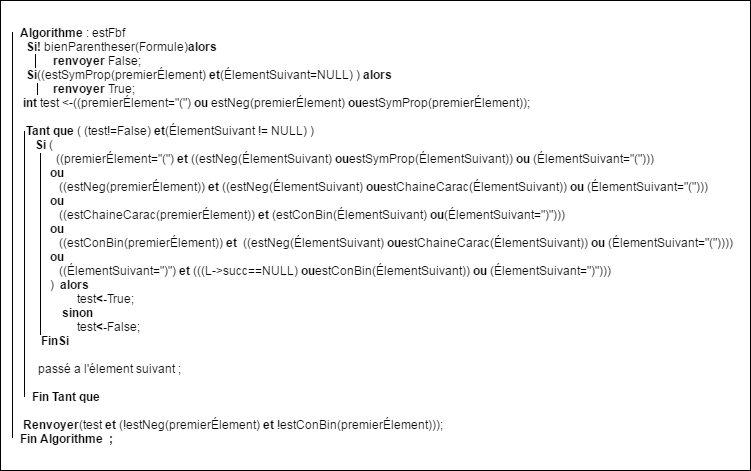
\includegraphics[width=150mm]{pm.png}
\subsubsection{La fonction qui permet de stocker les hypothèses et la conclusion  dans un abre \\ (Arbre* tabToArbre(char** T,int deb,int fin))}
Cette fonction va nous permettre de représenter une hypothèse ou une formule bien formée sous forme d'un arbre en respectant les règles de priorité pour les connecteurs binaires.\\
(Le non ($\neg$) est prioritaire sur le ou ($\vee$) qui est prioritaire sur l'implication ($\rightarrow$))\\

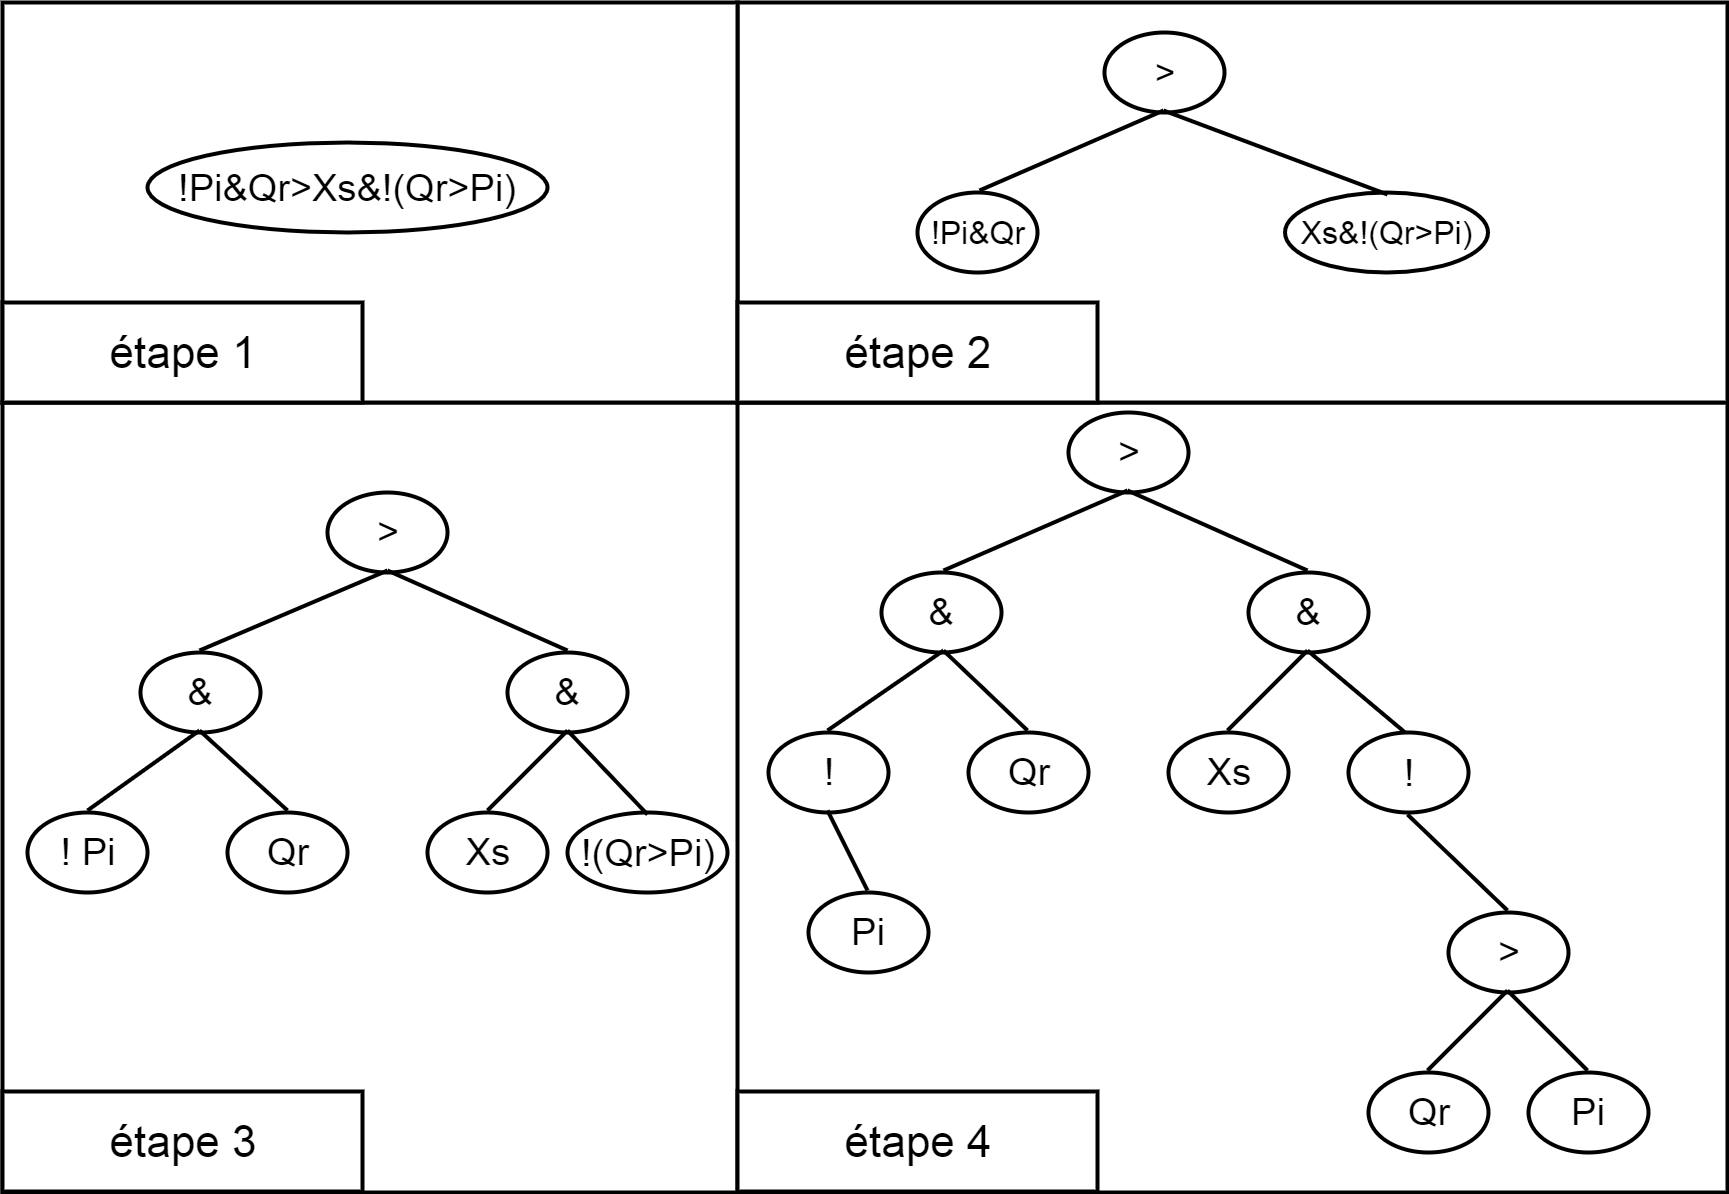
\includegraphics[width=130mm]{io.png}\\
Ceci est un exemple de l'application de la fonction.
\subsubsection{La fonction qui permet de réaliser les preuves \\ (void prouveurSequent(listeDeSequent *))}

Nous vérifions en premier lieu si la liste de séquent est vide. S'il elle est vide rien ne se passe,sinon on commence 
à prouver ce séquent.On teste chaque règle si elle est applicable ou pas.\\
Si plusieurs règles sont applicables alors l'entier (app) qui a été mis à 0 va nous permettre de savoir si on a déjà appliqué
une règle ou pas.Alors si app=1 cela veut dire qu'une règle a déjà été appliqué par conséquent aucune autre règle qui suit ne sera appliquée sur ce séquent.\\
Chaque fois qu'on applique la règle,on l'affiche le séquent initial et le séquent obtenu après l'application de cette règle.\\
La preuve se termine lorqu'on ne peut plus appliquer les règles sur un séquent ou lorqu'on arrive à prouver tous les séquents.



\section{Apport du projet}

Durant ce projet de 15 semaines, nous avons acquis beaucoup d'expérience tant en programmation qu'en conduite de projet.                               

\subsection{Apport scientifique et technique}
Ce projet nous à permis d'approfondir nos connaissances sur le sujet de la logique. Il nous à en premier lieu permis d'approfondir notre expérience sur le langance C. Aussi, ce projet a permis la connaissance de moyens de gestions de  projets tel que Gantt. De plus, on a exploré le domaine des interfaces graphiques (Gtk, Qt) qui sont des plus non négligeables dans notre apprentissage de l'informatique.

\subsection{Apport sur le gestion de projet}
                                              
Grace à ce projet, nous avons appris que le communication est un aspect primordiale pour la sérénité d'un projet.

Réussir à concevoir en vrai plutot que d'utiliser les moyens de messagerie permet du travail de meilleur qualité.


\section{Difficultés rencontrées}
Lors de ce projet nous avons rencontrés quelques difficultés dont :
\begin{itemize}
 \item Des difficultés avec le langage C# qui n'était pas bien maîtrisé par certains membres du groupe.
 \item Des difficultés en rédaction du rapport parce que tous les membres sont étrangés et personne n'a le français comme langue maternelle.
 \item Des difficultés de travail en groupe parce que certains membres habitent loin et ne peuvent pas rester tardivement à la faculté des sciences.
 \item Des difficultés sur la fonction qui permet de mettre des formules bien formées sous forme d'un arbre binaire.
\end{itemize}



 
\section{Annexe}
\appendix
\paragraph{BS1}
Antécédent:  R occurence dans les hypothèses

Conclusion: HYP $\vdash$ P $\rightarrow$ R

\paragraph{BS2}

Antécédent: P occurence dans les hypothèses

Conclusion: HYP $\vdash$ $\neg$P $\rightarrow$ R

\paragraph{DB1}

Antécédent: P occurence dans les hypothèses

Conclusion:  HYP $\vdash$ P

\paragraph{DB2}

Antécédent: $\neg$P occurence dans les hypothèses

Conclusion: HYP $\vdash$ P $\rightarrow$ R

\paragraph{DR1}

Antécédent:  HYP $\vdash$ P

Conclusion:  HYP $\vdash$ $\neg$ $\neg$P


\paragraph{DR2}

Antécédent: \begin{itemize}
             \item HYP $\vdash$ P
             \item HYP $\vdash$ $\neg$R
            \end{itemize}

Conclusion:  HYP $\vdash$ $\neg$(P $\rightarrow$ R)

\paragraph{DR3}

Antécédent: HYP $\vdash$ P $\rightarrow$ $\neg$ R

Conclusion: HYP $\vdash$ $\neg$(P $\wedge$ R)

\paragraph{DR4}

Antécédent: HYP $\vdash$ P $\rightarrow$ R

Conclusion: HYP $\vdash$ $\neg$ $\neg$P $\rightarrow$ R

\paragraph{DR5}

Antécédent:  HYP $\vdash$ P $\rightarrow$ ($\neg$Q $\rightarrow$ R)

Conclusion: HYP $\vdash$ $\neg$(P $\rightarrow$ Q) $\rightarrow$ R

\paragraph{DR6}

Antécédent: \begin{itemize}
             \item HYP $\vdash$ $\neg$P  $\rightarrow$ R
             \item HYP $\vdash$ $\neg$Q $\rightarrow$ R
            \end{itemize}

Conclusion: HYP $\vdash$  $\neg$(P $\wedge$ Q) $\rightarrow$ R

\paragraph{DR7}
 
Antécédent: \begin{itemize}
             \item HYP $\vdash$ $\neg$P  $\rightarrow$ R
             \item HYP $\vdash$ Q $\rightarrow$ R
            \end{itemize}
            
Conclusion: HYP $\vdash$  (P $\rightarrow$ Q) $\rightarrow$ R

\paragraph{DR8}
Antécédent: HYP $\vdash$  (P $\rightarrow$ Q) $\rightarrow$ R

Conclusion: HYP $\vdash$  P$\wedge$Q  $\rightarrow$ R

\paragraph{CNJ}
Antécédent: \begin{itemize}
             \item HYP $\vdash$ P
             \item HYP $\vdash$ $\neg$R
            \end{itemize}
            
Conclusion: HYP $\vdash$ P$\wedge$Q       

\paragraph{DED}
Antécédent: HYP,P $\vdash$ Q

Conclusion: HYP $\vdash$ P $\rightarrow$ Q
      


\section{Sources}
The B-Boook\\
Introduction à la logique par David Nour Raffalli
























































































































\end{document}    